%! Author = Eduardo Serna

% Preamble
\documentclass[twocolumn]{revtex4-2}

% Packages
\usepackage{amsmath}
\usepackage{graphicx} % For including images
\usepackage{hyperref} % For hyperlinks
\usepackage{amsfonts}
\usepackage{caption}
\usepackage{mathtools}

\newcommand{\bn}[1]{\mbox{\boldmath $#1$}}
\newcommand{\mb}{\mbox}
\newcommand{\angstrom}{\textup{\AA}}

% Document
\begin{document}

% Title Section
    \title{Weak Localization in Mono-layer Graphene with Rashba Spin-Orbit Interaction}
    \author{Eduardo Serna}
    \email{sernaed95@gmail.com}
    \affiliation{Centro de Investigación en Ciencias, Universidad Autónoma del Estado de Morelos, Morelos 62209, México}.
    \author{I. Rodríguez Vargas}
    \email{isaac@fisica.uaz.edu.mx}
    \affiliation{Unidad Académica de Física, Universidad Autónoma de Zacatecas, Zacatecas 98060, México}.
    \author{L. Diago-Cisneros}
    \email{ldiago@fisica.uh.cu}
    \affiliation{Facultad de Física, Universidad de La Habana, La Habana 10400, Cuba}.
    \date{26 December 2024}
    \maketitle

% Abstract
    \begin{abstract}
        Este trabajo estudia los efectos de la interacción espín-órbita tipo Rashba (SOIR) en el transporte de fermiones de Dirac en grafeno monocapa mediante paquetes de onda gaussianos.
        Se analiza la transmisión bajo distintas configuraciones de número de onda, energía y barrera de potencial.
        Los resultados muestran que la SOIR distorsiona significativamente los patrones de transmisión, revelando fenómenos como la ruptura de la degeneración de espín, la formación de estados cuasi-ligados y la dispersión dependiente del espín.

        Además, se propone un modelo para calcular la densidad de corriente de probabilidad considerando la interferencia de canales y efectos de auto-interferencia cuántica.
        Este modelo permite estudiar dinámicas de espín y diseñar dispositivos avanzados en espintrónica y computación cuántica.
        Los hallazgos destacan la relevancia de comprender y controlar la SOIR para optimizar el transporte cuántico en grafeno y potenciar aplicaciones en materiales bidimensionales.
    \end{abstract}

% Table of Contents (optional)
%    \tableofcontents
%    \newpage

% Introduction
    \section{Introduction}\label{sec:introduction}

        Monolayer graphene, a single layer of carbon atoms arranged in a honeycomb lattice, exhibits unique electronic properties stemming from quantum interference effects, spin-orbit interactions, and quantum dispersion.
        These properties are vital for potential applications in spintronics and quantum computing.

    \subsection{Weak Localization}\label{subsec:weak-localization}

        Weak localization (WL) and weak anti-localization (WAL) are quantum phenomena arising from the interference of electron waves in disordered materials.
         In graphene, these effects are heavily influenced by spin-orbit interactions (SOI), which describe the coupling between an electron's spin and its momentum.
          Strong SOI can cause a transition from WL to WAL, modifying the phase coherence length (the distance over which electron waves maintain their phase relationship) and impacting electrical conductivity\cite{WeizheMaterials2017,AvsarNatCommun2014}.
           This transition is crucial for understanding spin interactions within graphene and designing quantum devices.

    \subsection{Rashba-Type Spin-Orbit Interaction}\label{subsec:rashba-type-spin-orbit-interaction}

    Rashba-type SOI, originating from structural asymmetries in a material, can be significantly enhanced in graphene by proximity to other materials like transition metal dichalcogenides (TMDs) layered materials composed of a transition metal and two chalcogen atoms.
     This interaction introduces a strong SOI without altering graphene's structure\cite{WangPhysRevX2016, AvsarNatCommun2014}.
      The strength of this Rashba coupling affects phenomena such as spin-polarized-edge states (electrons at the material's edges possessing a preferred spin orientation) and is tunable using external electric fields.
      This tunability is a key advantage for spintronic applications.

    \subsection{Quantum Dispersion and Anomalous Hall Effect}\label{subsec:quantum-dispersion-and-anomalous-hall-effect}

    These interactions also impact quantum dispersion, the relationship between an electron's energy and momentum.
    The anomalous Hall effect (AHE), where a transverse voltage arises without an external magnetic field, has been observed in edge-bonded monolayer graphene\cite{LiuNano2023}.
     This demonstrates both ordinary and anomalous Hall effects, indicating long-range ferromagnetic order (spontaneous alignment of electron spins) and suggesting applications in carbon-based spintronics\cite{YaoMater2024}.
      The theoretical prediction of the quantum anomalous Hall (QAH) effect in graphene-based heterostructures further highlights the potential for hosting non-trivial topological phases.


    Electrostatic potential and Rashba spin-orbit interaction dramatically alter electron transmission in graphene, even at perpendicular incidence, defying the Klein paradox.
    The observed phenomenon results from several interacting factors: the creation of a classically forbidden region by the Potential, SOIR-induced spin degeneracy lifting and heavy hole effective mass alteration, spin-dependent interphase scattering, the formation of quasi-bound states leading to resonant tunneling, and the significant impact of the heavy hole effective mass on tunneling characteristics.
    These factors, particularly the deviation from the Dirac point dispersion relation, significantly modify transmission, requiring further computational and experimental investigation to fully elucidate this phenomenon and refine our understanding of graphene electron transport.

% Development
    \section{Development}\label{sec:development}
    \subsection{Physical Model}\label{subsec:physical-model}

We model a quantum channel formed by monolayer graphene (MLG) encapsulated on hexagonal boron nitride and capped with SiO$_2$.
Two metallic electrodes generate a perpendicular electric field that guides a Gaussian wave packet (GWP) along the channel.
A rectangular electrostatic barrier defines the scattering region where the SOIR is active.
Related setups and parameters are detailed in our previous article\cite{Serna2019}.

\subsection{Mathematical Model}\label{subsec:mathematical-model}

From the physical model, we can get a mathematical model which describes the temporal evolution and consequently the quantum dispersion of the Dirac fermions in the MLG\@.

Starting with the pristine graphene hamiltonian\cite{Geimk2007}:

\begin{equation}
    \label{eq:pristGr}
    \hat{\bn{H}}_G = v_{\mb{\tiny F}}\vec{\mathbf{\sigma}}\cdot\vec{p},
\end{equation}

\noindent With $\vec{\mathbf{\sigma}} = \hat{\mathbf{\sigma}}_{x}\hat{\imath} + \hat{\mathbf{\sigma}}_{y}\hat{\jmath}$, being the pseudospin Pauli matrices $\hat{\mathbf{\sigma}}_{x} = \bigl(\begin{smallmatrix}
0&1 \\ 1&0
\end{smallmatrix} \bigr)$, $\hat{\sigma}_{y} = \bigl(\begin{smallmatrix}
                                                         0&-i \\ i&0
\end{smallmatrix} \bigr)$, and $\vec{p}=\hat{p}_{x}\hat{\imath}+\hat{p}_{y}\hat{\jmath}$, the momentum operator, which $x, y$ components read $\hat{p}_{x} = -i\hbar\frac{\partial}{\partial x}$ and $\hat{p}_{y} = -i\hbar\frac{\partial}{\partial y}$, respectively.

The standard Rashba coupling for monolayer graphene (often written, in a four-component basis, as $\hat{H}_{\mathrm{DR}}=\lambda_R(\sigma_x s_y-\sigma_y s_x)$, with $s_i$ Pauli matrices in real-spin space) is generally very weak in pristine samples.

In our baseline configuration (pristine regions), we therefore neglect $\hat{H}_{\mathrm{DR}}$, consistent with typical estimates where $\lambda_R \ll \hbar v_F k_0$ and $\lambda_R \ll V_b$ at the scales of interest.

By contrast, in proximity-engineered heterostructures (e.g., graphene on TMDs or with Au), $\lambda_R$ can be enhanced to meV scales\cite{AvsarNatCommun2014, WangPhysRevX2016}.

In such cases, the canonical Dirac--Rashba term must be explicitly included in the Hamiltonian (together with the corresponding four-component spinor structure), and its consequences on wave-packet dynamics and transmission should be analyzed. We delineate this extension at the end of this subsection.


From this point forward, $v_{\mb{\tiny F}}$ stands for the Fermi velocity of the carriers in MLG, which satisfies

\begin{equation}
    \label{eq:vF}
    v_{\mb{\tiny F}} \approx \frac{c}{300}.
\end{equation}
This order-of-magnitude estimate is widely used for graphene\cite{Geimk2007}.

The previous Hamiltonian can be rewritten as:

\begin{equation}
    \label{eq:pristineGrapheneMatrix}
    \hat{\bn{H}}_G = -i\hbar v_{\mb{\tiny F}}
    \begin{pmatrix}
        0                                                         & \frac{\partial}{\partial x}- i\frac{\partial}{\partial y} \\
        \frac{\partial}{\partial x}+ i\frac{\partial}{\partial y} & 0
    \end{pmatrix}.
\end{equation}

Assuming that the momentum-dependent term of the Rashba Hamiltonian for Q1D (quasi-one dimensional) semiconductor hetero-structures can be extended to the context of MLG-Q1D\cite{RDiago2010, Serna2019, RCDiagoEPL2015}, it follows that the Hamiltonian for the SOIR can be written as:

\begin{equation}
    \label{eq:SOIRHamiltonian}
    \hat{\bn{H}}_R =
    \begin{pmatrix}
        0 & k_{\alpha-} + k_{\beta-} \\
        k_{\alpha+} + k_{\beta+} & 0
    \end{pmatrix},
\end{equation}

\noindent Where $k_{\alpha\pm} = \alpha\left(k_{\pm}^2/k_{\mp}\right)$ and $k_{\beta\pm} = \beta k_{\pm}^3$; also defining that $k_{\pm}=k_x\pm i k_y$ which are the initial wave numbers of the system.
The symbols $\alpha$ and $\beta$ represent the linear and cubic contribution of the SOIR respectively.

To calculate the values of the coupling constants $\alpha$ and $\beta$, we base our approach on the equations proposed by Wong and Mireles\cite{WongUNAM2005}:

\begin{align}
    \alpha &= \frac{eE_b P^2}{3E_i\left( E_i + E_g \right)}\label{eq: alfa}\\
    \beta &= -\frac{eE_b P^2\left( 2E_i + E_g \right)}{3E_i\left( E_i + E_g \right)^2 k_c^2}\label{eq: beta}\\
    E_i &= \frac{2P^2 k_c^2}{3E_g} \label{eq: E_i}\\
    \frac{2P^2}{m_0 E_g} &= \frac{m_0}{m^*} - 1 \label{eq: P2}\\
    E_b &= \frac{V_b}{el} \label{eq: E_b}
\end{align}

\noindent \textcolor{red}{where $e$ is the elementary charge, $P$ is the momentum matrix element, $E_g$ is the band gap, $k_c$ is a critical wave number that satisfies $k \ll k_c$, $m_0$ is the free-electron mass, $m^*$ is the effective mass used to parametrize the barrier region, $V_b$ is the barrier height, and $l$ is the barrier width.
In our modeling, carriers remain graphene electrons; the heavy-hole Rashba functional form is used only as an effective SOIR inside the barrier.}

Based on previous experimental data\cite{HuntSci2013, FuhrerSci2013, PallaBullMaterSci2016}, we define, as a reference, $E_g = 0.03$ eV and $m^* = 0.47m_0$; we also choose a critical wave number $k_c = 0.2$ \AA$^{-1}$ consistent with reported values.

If we substitute these numerical values, we can use~\eqref{eq: P2} to obtain $P^2=1.54\times10^{-32}$ kg$\cdot$eV; and, therefore, $E_i = 1.37\times10^{-32}$ eV\@.

Finally, we define the width and height of the barrier based on different physical models already presented in the literature.

Using these numerical results, we can find $\alpha$ and $\beta$.
For example, if $l=100$ \AA\, and $V_b = 0.5$ eV, then $\alpha = 0.25$ eV$\cdot$\AA\, and $\beta = -1.56$ eV$\cdot$\AA.

%alpha should be between 0.06 and 0.4 evA

%For monolayer graphene in contact with hexagonal Boron Nitride, approximately 30meV has been calculated

%We are also taking into account that $\alpha = -\beta$, following the conclusions presented by Wong and Mireles\cite{WongUNAM2005}.

For this research, we assume the heavy holes only in the region defined by the potential barrier.

The potential barrier is defined only in the specified region.

With the following Hamiltonian:

\begin{equation}
    \label{eq:potentialBarrierHamiltonian}
    \hat{\bn{H}}_V=\bn{I}_2 V(x)
\end{equation}

Adding up the graphene\eqref{eq:pristineGrapheneMatrix}, the SOIR\eqref{eq:SOIRHamiltonian}, and the potential barrier\eqref{eq:potentialBarrierHamiltonian} Hamiltonians, while also zeroing the parameters in the $y$ direction, we get:

\begin{equation}
    \label{eq:hybridHamiltonian}
    \hat{\bn{H}}=
    \begin{pmatrix}
        V(x) & \left(k_{\alpha-}+k_{\beta-}\right)-i\hbar v_{\mb{\tiny F}}\frac{\partial}{\partial x} \\
        \left(k_{\alpha+}+k_{\beta+}\right)-i\hbar v_{\mb{\tiny F}}\frac{\partial}{\partial x} & V(x)
    \end{pmatrix}.
\end{equation}

Note that if we wanted to see the results in the $y$ direction, we would have to zero the partial derivatives of $x$.

If the experimental context implies a giant Rashba coupling (e.g., proximity to TMDs, Au intercalation/adatoms), the Hamiltonian should be augmented to
(i) a four-component spinor (sublattice $\otimes$ real spin) and
(ii) include $\hat{H}_{\mathrm{DR}}=\lambda_R(\sigma_x s_y-\sigma_y s_x)$ along with $\hat{\bn{H}}_G$ and the electrostatic potential.
Within our time-evolution framework, this amounts to propagating a four-component Gaussian wave packet under the enlarged $4\times 4$ operator (the finite-difference machinery and stability criteria carry over directly).
Qualitatively, one should then expect pronounced spin splitting, spin precession inside and near the barrier, spin-dependent resonant features, and the possibility of transitions between Klein and anti-Klein tunneling regimes under suitable parameters\cite{DellAnnaJPhysCondMatt2018, AvsarNatCommun2014, WangPhysRevX2016}.

This is the basis of a more general model that can be explored in future work, particularly in light of recent experimental advances in engineering strong Rashba coupling in graphene-based heterostructures\cite{ManchonNatureMater2015}.

\subsection{Quasi-1D confinement and sub-band hybridization}\label{subsec:q1d-confinement-hybridization}
We model transport along $x$ under quasi-one-dimensional (Q1D) conditions produced by a transverse ($y$) electrostatic confinement that creates discrete transverse modes.
In practice, this can be achieved by electrostatic guiding (smooth $p$-$n$-$p$ profiles or split-gate definition) or narrow channels, leading to a ladder of sub-bands indexed by $n$ in the $y$ direction\cite{Young2009, ParedesPhysRevB2021, TrauzettelNature2007}.
Two limiting parametrizations are useful for estimates:
(i) hard-wall guiding of width $W$, where the transverse quantization gives $k_{y,n}\approx (n+\delta)\pi/W$ and a sub-band spacing $\Delta_y\sim \hbar v_F\pi/W$ between $n=0$ and $n=1$; and
(ii) approximately parabolic electrostatic confinement characterized by $\hbar\omega_y$, yielding a mode spacing $\Delta_y\simeq \hbar\omega_y$.

In our simulations, the barrier is uniform along $y$ (i.e., $V=V(x)$), and we set $\partial_y\to 0$ consistently with a single-mode approximation centered at $k_y\simeq 0$.
This is justified provided the injected Gaussian packet populates predominantly the lowest transverse mode, and inter-subband couplings are negligible.
Quantitatively, we impose the single-mode criteria
\begin{equation*}
\Delta_y \gg \max\{\lambda_R,\ \sigma_E,\ \hbar v_F\,\Delta k_y\},
\end{equation*}
\noindent where $\sigma_E$ is the energy spread of the packet and $\Delta k_y\sim 1/\sigma_y$ is its transverse-$k$ width (set by the real-space transverse width $\sigma_y$ of the injection).
For hard-wall guiding, this amounts to $\hbar v_F\pi/W \gg \{\lambda_R,\sigma_E,\hbar v_F/\sigma_y\}$; for smooth confinement, to $\hbar\omega_y \gg \{\lambda_R,\sigma_E,\hbar v_F/\sigma_y\}$.
Under these conditions, sub-band hybridization is suppressed and the Q1D reduction with $k_y\to 0$ (and $y$-derivatives zeroed) is controlled.

Sub-band hybridization can become important if (a) the confinement is weak (small $\Delta_y$ or wide $W$), (b) the wave packet significantly occupies multiple $k_y$ components, (c) the potential varies along $y$ (i.e., $V=V(x,y)$) producing mode-mixing matrix elements $\propto\langle n|\partial_y V|m\rangle$, or (d) spin-orbit terms couple modes with different transverse parity.
In such regimes, one must retain the full 2D problem or expand the spinor in transverse eigenmodes,
$\Psi(x,y,t)=\sum_n \chi_n(y)\, \varphi_n(x,t)$,
leading to coupled 1D channel equations with inter-mode couplings determined by $V(x,y)$ and Rashba matrix elements.
Hybridization then yields avoided crossings and multi-channel resonances in transmission (Fano-like features), and the effective single-channel picture no longer applies\cite{MiroshnichenkoRevModPhys2010}.

We have verified that the parameter sets used in this work satisfy the single-mode criteria above, ensuring that (i) only the lowest transverse mode is appreciably occupied at injection and (ii) inter-subband couplings driven by the barrier and Rashba terms remain negligible.
Consequently, the confinement term is justified and sub-band hybridization does not alter our conclusions within the explored parameter window.
Exploring multi-mode transport and intentional mode hybridization (e.g., by patterned $V(x,y)$ or stronger $\lambda_R$) is a natural extension of the present framework.

Note that if we wanted to see the results in the $y$ direction, we would have to zero the partial derivatives of $x$.

\subsection{Finite differences scheme}\label{subsec:finite-differences-scheme}

The main equation to solve is the time-dependent eigenvalue equation:

\begin{equation}
    \label{eq:schrodingerTimeDependent}
    i\hbar \frac{d}{dt}\bn{\Psi}(x,t) = \hat{\bn{H}}\bn{\Psi}(x,t)
\end{equation}

In our case, we consider a Gaussian wave packet (GWP) for each component of the pseudospinor $\bn{\Psi}(x,t)=\begin{psmallmatrix*}
\psi_A(x,t)\\\psi_B(x,t)
\end{psmallmatrix*}$.
The GWP at an initial time has the following form:

\begin{equation}
    \label{eq:GWP}
    \psi_j(x,t_0)=\frac{\xi_j}{\sqrt[4]{\pi\sigma^2}}e^{-\frac{(x-x_0)^2}{2\sigma^2}}e^{ixk_0}
\end{equation}

\noindent Where $\xi$ is the initial configuration of the pseudospinor, $k_0$ is the initial wave number in $x$, and the subscript $j$ indicates the component being used.

For the development of this article, we are using the following pseudospinor configuration options:

\begin{equation}
    \label{eq:pseudospinorConfigurations}
    \xi=\begin{pmatrix}
            1\\0
    \end{pmatrix},\,\,\begin{pmatrix}
                          1\\1
    \end{pmatrix},\,\,\begin{pmatrix}
                          1\\i
    \end{pmatrix},\,\,\begin{pmatrix}
                          1\\e^{i\pi/4}
    \end{pmatrix}.
\end{equation}

The wave packet is then defined as follows:

\begin{equation}
    \label{eq:FinalGWP}
    \bn{\Psi}(x,0)=\frac{1}{\sqrt {\xi_A^2 + \xi_B^2}}\begin{pmatrix}
                                                          \psi_A\\\psi_B
    \end{pmatrix}
\end{equation}

For the probability density calculated below, we use the following definition:

\begin{equation}
    \label{eq:probDens}
    \rho(x,t)=|\bn{\Psi}|^2 = |\psi_A|^2+|\psi_B|^2
\end{equation}

\subsection{Temporal Evolution Operator}\label{subsec:temporal-evolution-operator}
To solve the eigenvalue equation\eqref{eq:schrodingerTimeDependent}, we propose using a temporal evolution operator (TEO), based on the following equation:

\begin{equation}
    \label{eq:TEOdifEq}
    \bn{\Psi}(x,t)=\hat{U}(t,t_0)\bn{\Psi}(x,t_0)
\end{equation}

\noindent We can see that by applying the operator, we obtain a time $t$ from an initial time $t_0$.
If we substitute the TEO equation\eqref{eq:TEOdifEq} into the eigenvalue equation\eqref{eq:schrodingerTimeDependent}, we can develop the algebra and solve the differential equation to obtain the TEO\@.
Since the Hamiltonian does not depend on time, we can rewrite eq.\eqref{eq:TEOdifEq} as:

\begin{equation}
    \label{eq:TEOApplied}
    \bn{\Psi}(x,t)= e^{-\frac{i\delta t}{\hbar}\hat{\bn{H}}} \bn{\Psi}(x,t_0)
\end{equation}

\noindent Where $\delta t$ is the time step that we will discretize later.
The previous exponential can be approximated through the first-order Taylor series as:

\begin{equation}
    \label{eq:cayleyApprox}
    e^{-\frac{i\delta t}{\hbar}\hat{\bn{H}}} = \frac{2}{\bn{I} + \frac{i\delta t}{2\hbar}\hat{\bn{H}}}-\bn{I}
\end{equation}

Using a change of variable, we can rewrite the previous equation\eqref{eq:cayleyApprox} as:

\begin{equation}
    \label{eq:systemOfEquations}
    \bn{\Phi}(x,t_0) + \frac{i\delta t}{2\hbar}\hat{\bn{H}}\bn{\Phi}(x,t_0)=2\bn{\Psi}(x,t_0)
\end{equation}

\noindent This equation represents a system of $2\times2$ equations (since we have two unknowns, $\phi_A$ and $\phi_B$, and when developing the matrix, we can see that two equations are formed).

Since both equations have derivatives, we use the finite difference method to solve both equations for the entire space simultaneously.
To do this, we first discretize the system of equations\eqref{eq:systemOfEquations} along the entire space $j$ from $0$ to $J$.

To maintain the stability of the numerical analysis in the finite difference method, the following condition must be respected\cite{Carrillo2015}:

\begin{equation}
    \label{eq:stabilityCondition}
    \delta t \leq \frac{\left( \delta x \right)^2}{2}
\end{equation}

To discretize the derivatives, we use the Taylor series expansion up to the first degree for the point $x_j$ forward and backward:

\begin{align}
    \label{eq:TaylorBeforeAndAfter}
    f(x_j+\delta x)&=f(x_j) + (x_j+\delta x-x_j)f'(x_j)\nonumber\\
    &=f(x_j)+\delta xf'(x_j),\nonumber\\
    f(x_j-\delta x)&=f(x_j) + (x_j-\delta x-x_j)f'(x_j)\nonumber\\
    &=f(x_j)-\delta xf'(x_j),
\end{align}

\noindent if we subtract the second equation from the first and solve for $f'(x_j)$, we can find the ``Central Differences'' which we can also discretize as:

\begin{equation}
    \label{eq:diferenciasCentradas}
    f'(x_j)=\frac{f(x_j+\delta x)-f(x_j-\delta x)}{2\delta x} = \frac{f_{j+1}-f_{j-1}}{2\delta x}
\end{equation}

In this way, we can rewrite our system of equations, once the discretization and algebraic development of the matrix have been performed:

\begin{multline}
    \label{eq:partA}
    \phi_{A, j} + \frac{i\delta t}{2\hbar}(V_j\phi_{A,j} + \left(k_{\alpha-,j}+k_{\beta-,j}\right)\phi_{B,j}-\\
    i\hbar v_{\mb{\tiny F}}\frac{\phi_{B, j+1}-\phi_{B, j-1}}{2\delta x}) = 2\psi_{A,j}
\end{multline}

\begin{multline}
    \label{eq:partB}
    \phi_{B, j} + \frac{i\delta t}{2\hbar}(V_j\phi_{B,j} + \left(k_{\alpha+,j}+k_{\beta+,j}\right)\phi_{A,j}-\\
    i\hbar v_{\mb{\tiny F}}\frac{\phi_{A, j+1}-\phi_{A, j-1}}{2\delta x}) = 2\psi_{B,j}
\end{multline}

If we add Eq.\eqref{eq:partA} and Eq.\eqref{eq:partB}:


\begin{align}
    \label{eq:temporaryEquation}
    2\begin{pmatrix}
         \psi_{A,1} + \psi_{B,1} \\
         \psi_{A,2} + \psi_{B,2} \\
         \vdots                  \\
         \psi_{A,J} + \psi_{B,J} \\
    \end{pmatrix} &=
    \begin{pmatrix}
        N      & Q      & 0      & \ldots & \ldots & \ldots & 0 \\
        -Q     & N      & Q      & 0      & \ldots & \ldots & 0 \\
        0      & -Q     & N      & Q      & 0      & \ldots & 0 \\
        \vdots & 0      & -Q     & N      & Q      & \ddots & 0 \\
        \vdots & \vdots & 0      & -Q     & N      & \ddots & 0 \\
        \vdots & \vdots & \vdots & \ddots & \ddots & \ddots & Q \\
        0      & 0      & 0      & 0      & 0      & -Q     & N
    \end{pmatrix}\begin{pmatrix}
                     \phi_{A,1} \\
                     \phi_{A,2} \\
                     \vdots     \\
                     \phi_{A,J}
    \end{pmatrix}\\
    &+\begin{pmatrix}
          M      & Q      & 0      & \ldots & \ldots & \ldots & 0 \\
          -Q     & M      & Q      & 0      & \ldots & \ldots & 0 \\
          0      & -Q     & M      & Q      & 0      & \ldots & 0 \\
          \vdots & 0      & -Q     & M      & Q      & \ddots & 0 \\
          \vdots & \vdots & 0      & -Q     & M      & \ddots & 0 \\
          \vdots & \vdots & \vdots & \ddots & \ddots & \ddots & Q \\
          0      & 0      & 0      & 0      & 0      & -Q     & M
    \end{pmatrix}\begin{pmatrix}
                     \phi_{B,1} \\
                     \phi_{B,2} \\
                     \vdots     \\
                     \phi_{B,J}
    \end{pmatrix}
\end{align}


\noindent where $N =1 + \frac{i\delta t}{2\hbar} \left( V_j + \left(k_{\alpha+,j}+k_{\beta+,j}\right)\right)$, $Q=\frac{i\hbar v_{\mb{\tiny F}}}{2\delta x}$ and $M =1 + \frac{i\delta t}{2\hbar}\left( V_j + \left(k_{\alpha-,j}+k_{\beta-,j}\right)\right)$.

As can be seen, the size of the matrix depends on the size of our system.
If we choose $\delta x = 1\angstrom$, then a quantum well of $1200\angstrom$ will generate a matrix of $1200\times1200$.

We repeat the previous procedure but now subtracting Eq.\eqref{eq:partA} and Eq.\eqref{eq:partB}

Looking at these matrices, we can redefine them as two simple matrix equations $2\psi_+=\mathbb{N}\phi_A+\mathbb{M}\phi_B$ and $2\psi_-=\mathbb{L}\phi_A+\mathbb{P}\phi_B$.
These equations can be treated as a system of matrix equations that are solved as follows:

\begin{align}
    \label{eq:sistemaMatricial}
    \phi_A&=(2\mathbb{N}^{-1})\psi_+-(\mathbb{N}^{-1}\mathbb{M})\phi_B\nonumber\\
    \phi_B&=2(-\mathbb{L}\mathbb{N}^{-1}\mathbb{M}+\mathbb{P})^{-1}(\psi_--\mathbb{L}\mathbb{N}^{-1}\psi_+)
\end{align}

Once we have the discretized system of equations, the temporal evolution can be calculated with:

\begin{equation}
    \label{eq:siguienteTiempo}
    \Psi_j^{n+1}=\Phi_j^n-\Psi_j^n
\end{equation}

Repeating the process for each $n$ until reaching $N$.

\subsection{Probability Current Density}\label{subsec:probability-current-density}

Once we have the temporal evolution, we can calculate its transmission coefficient from the calculation of the probability current density (PCD).
To find this current, we start from the following continuity equation:

\begin{equation}
    \label{eq:continuidad}
    \frac{\partial\rho}{\partial t} + \nabla\cdot\vec{j}=0
\end{equation}

Applying the conjugate transpose to the time-dependent eigenvalue equation\eqref{eq:schrodingerTimeDependent}, and multiplying on the right by $\Psi$, we can incorporate the probability density equation\eqref{eq:probDens}.
At the same time, we consider the graphene Hamiltonian\eqref{eq:pristGr}, which we know is Hermitian since it is composed of Pauli matrices.
In this way, we can construct the following equation:

\begin{equation}
    \label{eq:rho_sigma_nabla}
    \frac{\partial}{\partial t}\int\rho d\vec{r} = -v_f\int\left( \Psi\vec{\sigma}\cdot\nabla\Psi^{T*} + \Psi^{T*}\vec{\sigma}\cdot\nabla\Psi \right)d\vec{r}
\end{equation}

We can rewrite the equation by factoring out $\nabla$ and removing the integral from both sides:

\begin{equation}
    \label{eq:casi_j}
    \frac{\partial}{\partial t}\rho = -v_f\nabla\cdot\left( \Psi^\dagger \vec{\sigma} \Psi \right)
\end{equation}

Substituting into the continuity equation of probability density eq.\eqref{eq:continuidad}:

\begin{equation}
    \label{eq:nablaJ}
    \nabla\cdot\vec{j} = v_f\nabla\cdot\left( \Psi^\dagger \vec{\sigma} \Psi \right)
\end{equation}

Eliminating $\nabla$ from both sides:

\begin{equation}
    \label{eq:final}
    \vec{j} = v_f\Psi^\dagger \vec{\sigma} \Psi
\end{equation}

In this way, we have obtained the probability current density in graphene.

If we want to obtain the components of the current density, we can do it as follows:

\begin{equation}
    \label{eq:componentes}
    \vec{j} = v_f\begin{pmatrix}
                     \Psi^\dagger \sigma_x \Psi \\ \Psi^\dagger \sigma_y \Psi
    \end{pmatrix} = v_f\begin{pmatrix}
                           \Psi_A^\dagger\Psi_B + \Psi_B^\dagger\Psi_A \\ i(-\Psi_A^\dagger\Psi_B + \Psi_B^\dagger\Psi_A)
    \end{pmatrix}
\end{equation}

The importance of the current vector expression, shown explicitly in equation\eqref{eq:componentes}, lies in the detailed understanding of the pseudospin behavior of graphene.
The clear characterization of both components of the current vector is central to interpreting the numerical results and understanding the phenomenology associated with transport in these structures.

As a verification, if we consider an incident plane wave function, we can express it as:

\begin{equation}
    \label{eq:ondaPlana}
    \Psi(\vec{r})=\frac{e^{i\vec{k}\cdot\vec{r}}}{\sqrt{2}}
    \begin{pmatrix}
        1 \\ e^{i\theta}
    \end{pmatrix},
\end{equation}

\noindent where $\theta$ is the angle of incidence with respect to the direction normal to the barrier and $\vec{k} = k(\cos\theta,\sin\theta)$ is the wave vector.

If we substitute eq.\eqref{eq:ondaPlana} into eq.\eqref{eq:componentes}, we can simply perform the multiplication as follows to obtain the probability current density incident on the barrier along the $X$ axis ($j_{x,in}$):

\begin{align}
    \label{eq:jdemostrada}
    j_{x, in}&=v_f\frac{1}{2}
    \begin{pmatrix}
        e^{-i\theta} & 1
    \end{pmatrix}
    \begin{pmatrix}
        0 & 1 \\
        1 & 0
    \end{pmatrix}
    \begin{pmatrix}
        1 \\ e^{i\theta}
    \end{pmatrix}\nonumber \\
    &=v_f\left( \frac{e^{-i\theta} + e^{i\theta}}{2} \right)\nonumber \\
    &=v_f\cos\theta
\end{align}

This simplification is what is commonly used in the literature\cite{DahalJPhysChemSolids2017, WuJAP2009}.

To determine the numerical value of $\vec{\jmath}$, we identify the peaks in the probability density plots.
Subsequently, we calculate the minima of the Gaussian curves to find the apparent width of the GWP. Finally, we locate two precise moments: immediately before the wave packet interacts with the potential barrier and the exact moment it has traversed the barrier.

With the defined entry ($t_1$) and exit ($t_2$) times, we use Eq.\eqref{eq:componentes} for the entire space at each of these times.

With this, we can now calculate the transmission coefficient:

\begin{equation}
    \label{eq:transmissionCoef}
    T = \left| \frac{\vec{\jmath}_{out}\cdot\hat{n}}{\vec{\jmath}_{in}\cdot\hat{n}} \right|,
\end{equation}

\noindent In this context, the ratio between the transmitted current and the incident current is calculated, considering the product with the vector normal to the barrier.
In the one-dimensional case addressed here, this vector can be represented as $(1,0)$ or $(0,1)$, depending on whether the Gaussian wave packet (GWP) propagates along the $x$-axis or the $y$-axis, respectively.

Having presented the conceptual framework and the fundamental equations of the studied system, we now proceed with the analysis and critical discussion of the results obtained through numerical simulations.
This section will allow us to evaluate and contrast in detail the influence of the Rashba term on quantum transmission in monolayer graphene.


    \section{Discussion of Results}\label{sec:discussion-of-results}

    A continuación se muestran las figuras obtenidas con el procedimiento obtenido anteriormente.

    \begin{figure}[h!]
        \centering
        \begin{minipage}[t]{0.48\textwidth}
            \centering
            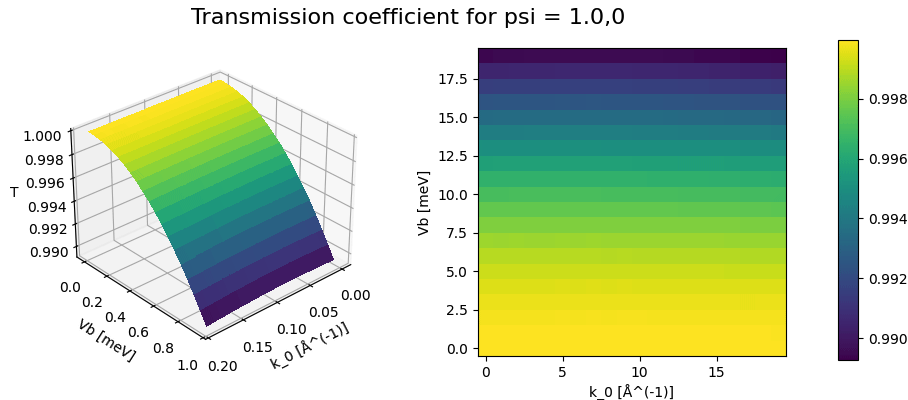
\includegraphics[width=\textwidth]{../assets/images/No-Rashba/TCoefficient(1.0,0)xalpha=0beta=0}
            \captionof{figure}{Transmisión en grafeno prístino.
            En el eje vertical vemos el coeficiente de transmisión, y en el plano está la intensidad de la barrera de potencial en meV contra el número de onda inicial $\angstrom^{-1}$.
            Podemos ver que el coeficiente de transmisión se mantiene constante a lo largo de los diferentes valores de $k$, sin embargo, conforme la barrera de potencial aumenta, el coeficiente de transmisión disminuye.
            Desde $1$ hasta $0.990$.}
            \label{fig:noRashba}
        \end{minipage}
        \hfill
        \begin{minipage}[t]{0.48\textwidth}
            \centering
            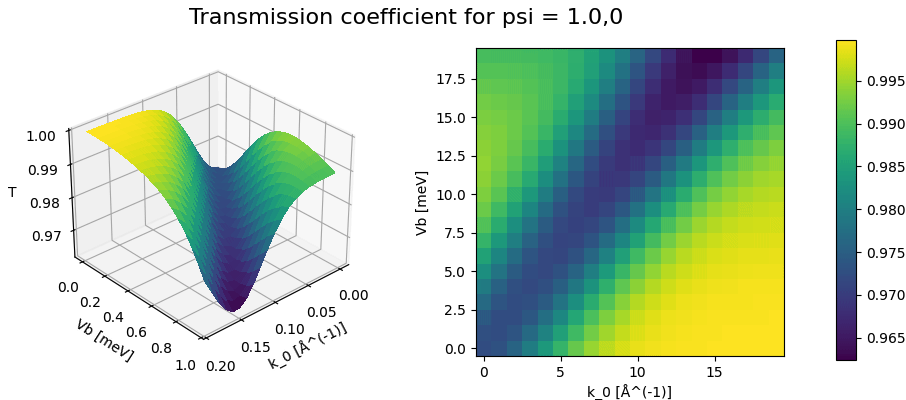
\includegraphics[width=\textwidth]{../assets/images/Rashba/TCoefficient(1.0,0)xalpha=0.2beta=-0.2}
            \captionof{figure}{Transmisión considerando SOIR en la zona de la barrera de potencial.
            En este caso se observa que el coeficiente de transmisión varía drásticamente formando un patrón similar a una hoja semi-doblada.
            En el mapa de colores se observa claramente una tendencia.}
            \label{fig:rashba}
        \end{minipage}
    \end{figure}

    En las imágenes podemos notar ciertas aspectos interesantes, empezando con la fig.\ref{fig:noRashba}.
    Esta figura muestra una caída del coeficiente de transmisión conforme la intensidad de la barrera de potencial aumenta.
    Este resultado muestra una contradicción con lo que ya se especifíca en la literatura, en el grafeno se esperaría observar una transmisión total debido a las mismas propiedades del material\cite{horsell2008, Young2009}.

    The observed behavior might be the result of one or both of the following aspects:

    \begin{itemize}
        \item Wave Packet Characteristics:
        Not a single momentum eigenstate.
        Debido a que estamos ocupando paquetes de onda en la simulación, un detalle importante que surge es que existe la presencia de múltiples componentes de momentum y eso implica que algunos de ellos pueden causar interferencia con otros; causando un coeficiente de transmisión que difiere del de un sólo autoestado\cite{Staelens2021}.
        Además, en nuestra simulación se está tomando en cuenta el tiempo.
        Parte de la investigación a futuro es comprobar si el tiempo de fase o de tunelaje están directamente relacionados a la variación del coeficiente de transmisión observada en este trabajo.
        \item Quantum interference effects\cite{MolgadoMex2018}.
        Dependiendo del ancho del paquete y su amplitud, éste se puede dispersar con el tiempo y esto puede causar interferencia con sí mismo.
        Conforme diferentes partes del GWP encuentran la barrera de potencial, estos pueden estar interfiriendo, causando fluctuaciones en el coeficiente de transmisión.
    \end{itemize}

    Por otro lado, tenemos la transmisión bajo presencia de SOIR (Fig.\ref{fig:rashba}).
    Es evidente que se forma una correlación: a mayor altura de la barrera de potencial y mayor el número de onda inicial del paquete de ondas, entonces menor será la transmisión.
    Sin embargo, el comportamiento interesante aquí es que conforme el valor de $k_0$ sea mayor, y $V_b$ sea menor; entonces se obtiene una transmisión más cercana a $1$.

    A pesar de que la variación en el coeficiente de transmisión es mínima (del orden de $10^{-2}$), esta variación se podría explicar por la misma SOIR, los electrones con diferentes componentes del pseudoespinor interactúan con los de la otra componente.
    Como ya se había observado antes\cite{Serna2019}, la SOIR puede variar por el número de onda inicial del GWP, de ahí se puede deducir que esta interacción causa la variación en el coeficiente de transmisión.


% Conclusions
    \section{Conclusions}\label{sec:conclusions}

Este trabajo analiza, teórica y computacionalmente, los efectos del acoplamiento espín-órbita tipo Rashba (SOIR) en la transmisión de electrones a través de una barrera de potencial en grafeno monocapa.
Los resultados muestran que el SOIR altera significativamente los coeficientes de transmisión, generando patrones ausentes en grafeno prístino.
Esto se debe posiblemente a la interacción entre el pseudoespinor de los electrones.

En grafeno prístino sin SOIR, la transmisión permanece cercana a la unidad, como se espera por la supresión del retroceso de electrones.
Sin embargo, se observan pequeñas caídas en la transmisión por interferencias cuánticas en el paquete de onda gaussiano utilizado.
Estas interferencias resaltan la sensibilidad del sistema y la necesidad de estudiar la relación entre el tiempo de fase y las propiedades de transporte.

Con SOIR, emergen patrones complejos de transmisión relacionados con los parámetros de la barrera y el paquete de ondas, atribuibles a fenómenos como el levantamiento de la degeneración de espín y la dispersión espín-dependiente.
Estos resultados subrayan la relevancia del SOIR para diseñar dispositivos cuánticos avanzados con aplicaciones en spintrónica y computación cuántica.

%% Acknowledgments
%    \section*{Acknowledgments}

% References
    \bibliographystyle{apsrev4-2}
    \bibliography{/Users/Serkne/WebstormProjects/MLGQ1DWL/bib/main}

\end{document}